\appendix

\chapter{Figures}

\begin{figure}
    \centering
    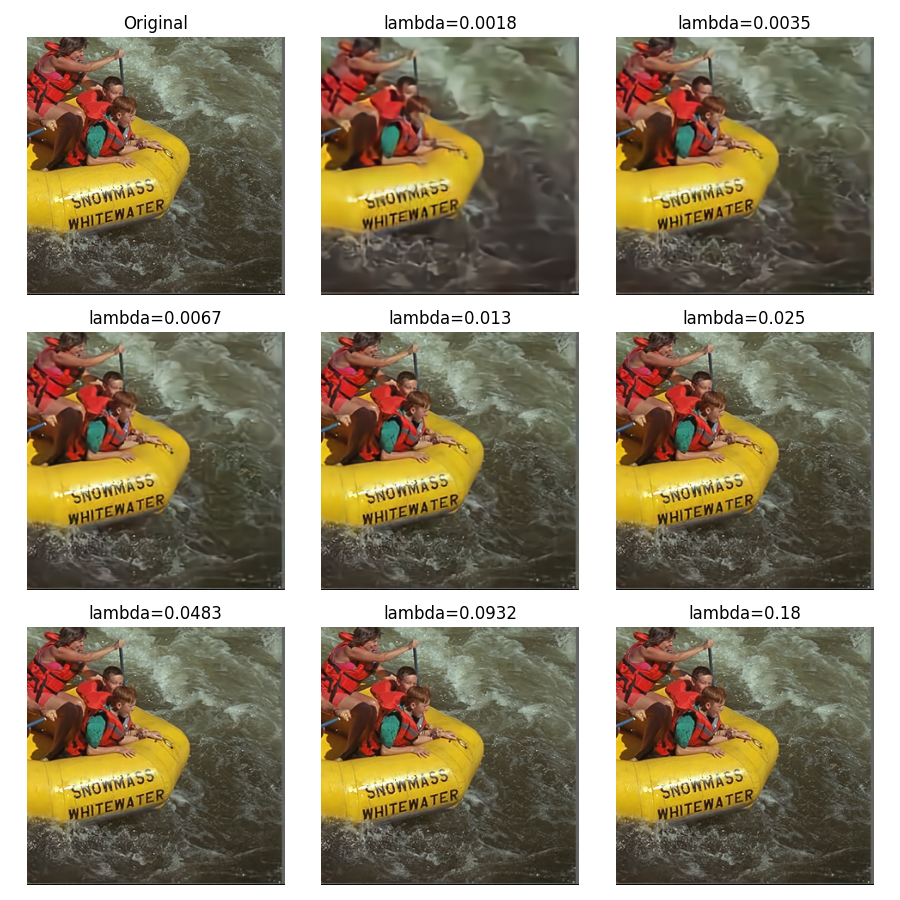
\includegraphics[width=15cm]{img/balle_bdpsnr_1a.png}
    \caption{Reconstruction results on image 14 of the Kodak dataset using our networks}
    \label{bdpsnr_1a_app}
\end{figure}

\begin{figure}
    \centering
    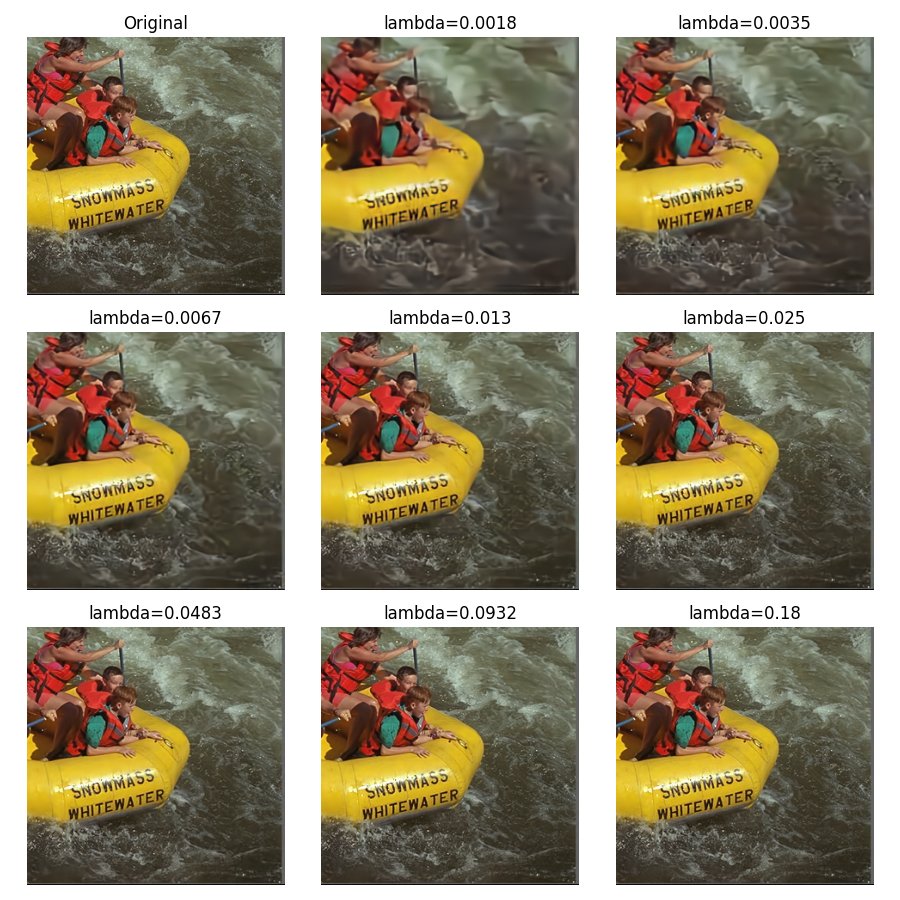
\includegraphics[width=15cm]{img/balle_bdpsnr_1b.png}
    \caption{Reconstruction results on image 14 of the Kodak dataset using pre-trained networks}
    \label{bdpsnr_1b_app}
\end{figure}

\begin{figure}
    \centering
    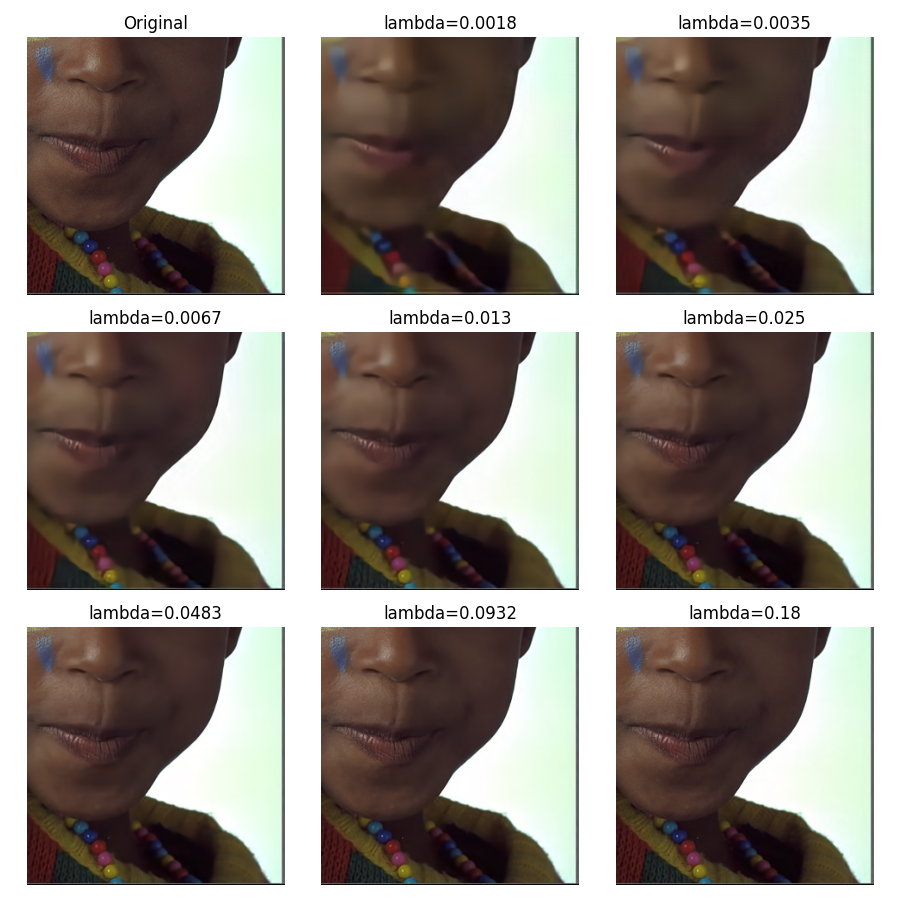
\includegraphics[width=15cm]{img/balle_bdpsnr_2a.png}
    \caption{Reconstruction results on image 15 of the Kodak dataset using our networks}
    \label{bdpsnr_2a_app}
\end{figure}

\begin{figure}
    \centering
    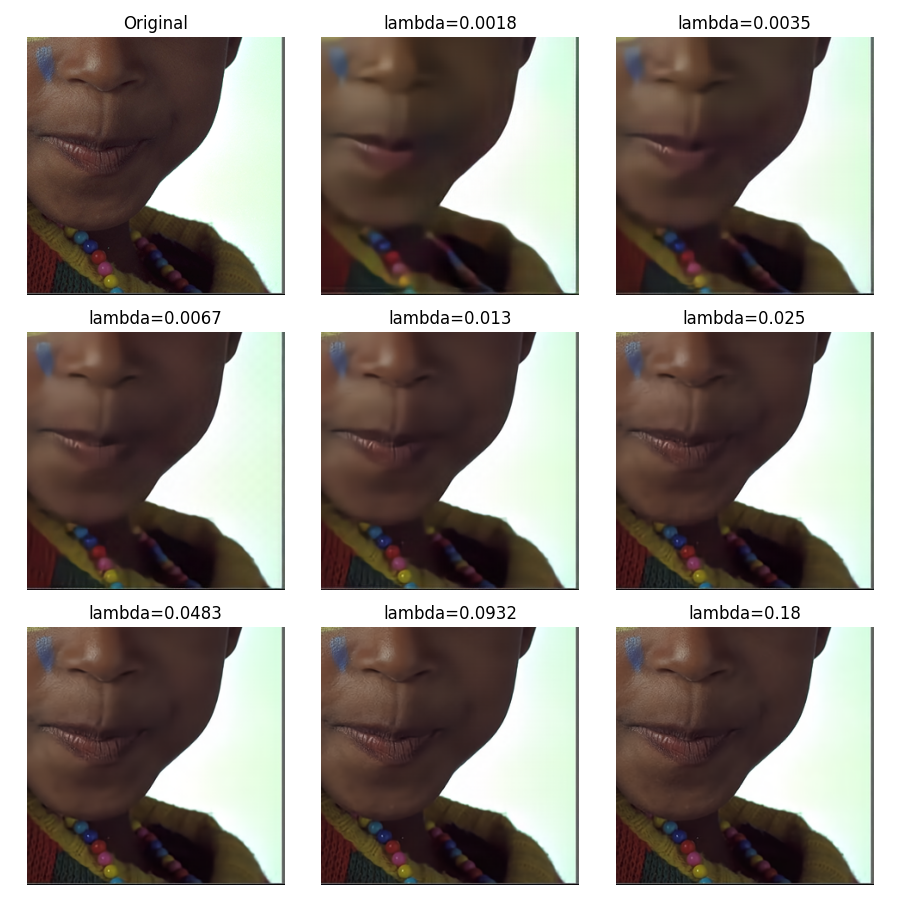
\includegraphics[width=15cm]{img/balle_bdpsnr_2b.png}
    \caption{Reconstruction results on image 15 of the Kodak dataset using pre-trained networks}
    \label{bdpsnr_2b_app}
\end{figure}

\chapter{Implementation Details}
Here is a list of useful details regarding our implementation:
\begin{itemize}
    \item Python 3.12.7
    \item Anaconda virtual environment
    \item compressAI 1.2.6
    \item Code hosted on private GitHub repository
    \item Processing power provided by Télécom Paris GPU cluster (\url{https://docs.google.com/document/d/1lXykfpEUJCrbNh22D2f2kxNS0gV6t-j9A_juWFdiEnI/edit?tab=t.0})
\end{itemize}